% Send to Mandar,Jayesh,Arnab,Deepak and perhaps Rahee, PEB, AAO, Michael Richards, John W, Jaydeep K, and Grace Gu, GR Gogate, Chaitanya Bapat, Ruhi
\documentclass[12pt]{article}
\newcommand{\beq}{\begin{equation}}
\newcommand{\eeq}{\end{equation}}
\newcommand{\ber}{\begin{eqnarray}}
\newcommand{\eer}{\end{eqnarray}}
\newcommand{\nn}{\nonumber}
\newcommand{\dd}[2]{\frac{d}{d{#2}}{(#1)} }
\newcommand{\pdd}[2]{\frac{\partial}{\partial{#2}}{(#1)} }
\usepackage{amsmath}
\usepackage{amsfonts}
\usepackage{cite}
\usepackage{url}
\usepackage{graphicx}
\usepackage{caption}
\usepackage{subcaption}
\usepackage{multirow}
\usepackage{draftwatermark}
\SetWatermarkText{Draft}
\SetWatermarkScale{5}
%
\begin{document}
% bib
\title{Initial elasticity imaging results using a Convolutional Neural Network}
\author{Nachiket Gokhale\footnote{The author is very grateful to Paul Barbone for patiently answering many questions about finite elements. Conversations with Arnab Majumdar, Michael Richards and Mandar Kulkarni are gratefully acknowledged and appreciated.}\\gokhalen@gmail.com}
\date{\today}
\maketitle
\abstract{We explore the application of a Convolutional Neural Network (CNN) using labeled data (supervised learning) to image the shear modulus field of an almost incompressible elastic medium using displacement or strain field data. This problem is important in medicine because the shear modulus of suspicious and potentially cancerous growths in soft tissue is elevated by about an order of magnitude as compared to the background of normal tissue. Therefore, imaging the stiffness leads to high-contrast medical images. Our prediction problem is as follows: Given displacement or strain fields, predict the shear modulus field. Our CNN is trained using 2400 training examples consist of displacement or strain fields and a corresponding shear modulus field. We present encouraging results which warrant further research and show the promise of this methodology.}
\section{Introduction}
The shear modulus of palpable nodules (which can be thought of as abnormal and potentially cancerous growths in soft tissue) is approximately an order of magnitude higher than the stiffness of the background of normal glandular tissue \cite{paper:sarv1998}. See also Figure (\ref{fig:shearmod}). It follows then, that imaging the shear modulus of soft tissue results in a high-contrast imaging method because suspicious growths will stand out clearly against the background of normal tissue. Elasticity Imaging is a broad term that refers to methods which image the shear modulus (or other elastic properties) of soft tissue in various ways. Elasticity Imaging typically consists of  the following steps:
%
\begin{figure}
   \centering
    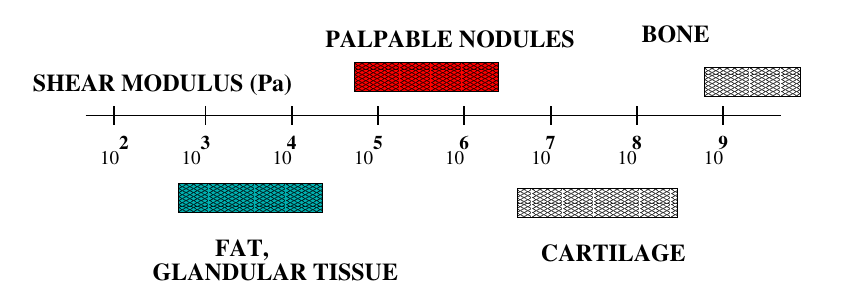
\includegraphics[totalheight=3cm]{Figures/shearmod.png}
  \caption{\label{fig:shearmod} Shear moduli of different types of soft tissue. Adapted from Figure 1 in \cite{paper:sarv1998}.}
\end{figure}
%
\begin{enumerate}
\item{\textbf{Image acquisition:} Images of soft tissue undergoing deformation are acquired using various imaging modalities such as ultrasound or magnetic resonance imaging. While time dependent images can be acquired, we shall consider here only two images: a \textit{pre-deformation image} acquired before force is applied and a \textit{post-deformation image} acquired after force is applied. This process is shown in Figure (\ref{fig:prepostimage}) for ultrasound imaging.}
\item{\textbf{Image registration:} The goal in this step is to find a map between the \textit{pre-deformation image} and the \textit{post-deformation image}. For every point in the \textit{pre-deformation image} we aim to find its location in the \textit{post-deformation image}. This gives us the \textit{displacement field} between the two images. This displacement field is often referred to as the \textit{measured displacement field}.}
\item{\textbf{Inverse problem solution:} The goal in this step is to infer the spatial distribution of the shear modulus from the displacement field. The approaches can be divided into two categories: direct and iterative. Direct approaches involve solving a partial differential equation (pde) to obtain the distribution of shear modulus directly (cite Kallel Bertrand,Oberai). Such approaches work well when the measured strain field is completely known and has low noise. Iterative approaches (cite Doyley, Oberai ) involve guessing a distribution for the shear modulus, solving a linear elasticity forward problem to obtain the predicted displacements, comparing the predicted displacements to the measured displacements and updating the guessed shear modulus distribution using a suitable optimization procedure such as Gauss-Newton (cite Marvin's paper) or BFGS ( as in cite my paper).}
\end{enumerate}
%
\begin{figure}
   \centering
    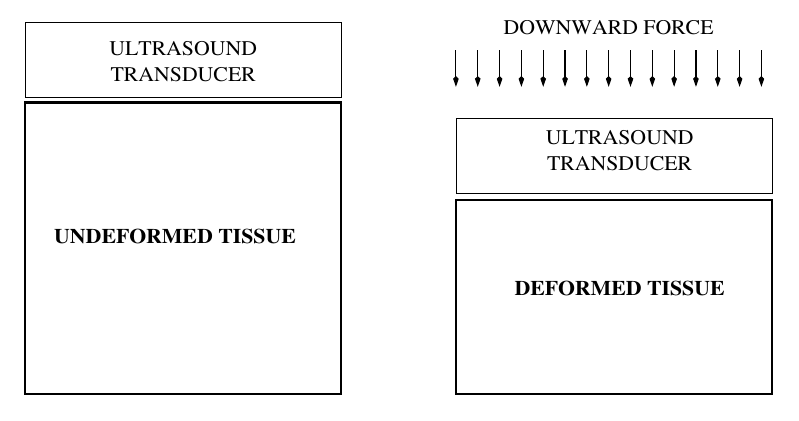
\includegraphics[totalheight=5cm]{Figures/prepostimage.png}
  \caption{\label{fig:prepostimage} Schematic figure showing medical image acquisition when soft tissue is being deformed using ultrasound imaging.}
\end{figure}
%
\section{Neural Networks}
In recent years, Neural Networks have been applied to various applications such as image classificaton \cite{paper:hinton2017}, hand written digit recognition \cite{paper:kulkarni2018}, solving differential equations and symbolic integration \cite{misc:lample2019}, solving complex partial differential equations such as the Navier-Stokes equation \cite{misc:anandkumar2020}, self-driving cars \cite{misc:agnihotri2019,misc:nvidiaselfdriving2016}, chaos . Several effective Machine Learning frameworks such as Google's TensorFlow \cite{misc:tensorflow}, Facebook's PyTorch \cite{incollect:pytorch}, Scikit-Learn \cite{paper:scikit-learn} are freely available. See \url{https://en.wikipedia.org/wiki/Comparison_of_deep-learning_software} for a complete list.
%
\section{Problem definition}
\section{Binary classification}
% https://stackoverflow.com/questions/31324218/scikit-learn-how-to-obtain-true-positive-true-negative-false-positive-and-fal

%By definition a confusion matrix C is such that C[i, j] is equal to the number of observations known to be in group i but predicted to be in group j.

%Thus in binary classification, the count of true negatives is C[0,0], false negatives is C[1,0], true positives is C[1,1] and false positives is C[0,1].

% CM = confusion_matrix(y_true, y_pred)

% TN = CM[0][0]
% FN = CM[1][0]
% TP = CM[1][1]
% FP = CM[0][1]

\section{Things to do}
% Custom activation function
% https://stackoverflow.com/questions/43915482/how-do-you-create-a-custom-activation-function-with-keras
\begin{enumerate}
\item{Checkpoint and save best weights instead of just running for $512$ epochs. https://stackoverflow.com/questions/42666046/loading-a-trained-keras-model-and-continue-training}
\item{Also, checkpoint and restart}
\item{}
\item{Use prior knowledge to improve performance. e.g. if we know that radius can lie between 1 pixel and 3 pixels, perhaps we can use that information to improve performance. Similarly if we know that stiffness can lie between specifed ranges, then use that knowledge to constrain NN output}
\item{Better results are obtained for larger inclusion with larger contrast}
\item{Larger datasets: 100,000 or so datasets}
\item{Better NN architectures}
\item{Mapping medical images to shear modulus directly skipping registration.}
\item{Training multiple NNs on the same data set using different initializations for the weights. One can then average the prediction or average the weights.}
\item{Handling noise: augmenting dataset by adding noise to displacement/strain fields}
\item{Stiffness is always underpredicted. Smaller inclusions are not handled well. Larger inclusions are handled better.}
\item{Actual material properties and breast/organ geometry}
\item{Multiple displacement fields}
\end{enumerate}
\bibliography{eibib}{}
\bibliographystyle{plain}
\end{document}
